\documentclass[10pt,a4paper]{article}
\usepackage[latin1]{inputenc}
\usepackage{amsmath}
\usepackage{amsfonts}
\usepackage{amssymb}
\usepackage{graphicx}

%%% formatting the code
\usepackage{listings}
\usepackage{color}
\lstset{%
	escapeinside={(*}{*)},%
}

\newcommand{\amidstversion}{\input{../../version.txt}}


\usepackage{hyperref}

\begin{document}

\section{Basic steps for
	contributing}\label{basic-steps-for-contributing}

Here we will explain the basic github commands for modifying the AMIDST
source code and for uploading such changes to the server. Alternatively,
you can watch this
\href{https://www.youtube.com/watch?v=HegfZZyQ8u4}{video-tutorial}. The
general scheme to follow for contributing to the AMIDST source code is
shown below:

\begin{figure}[h!]
	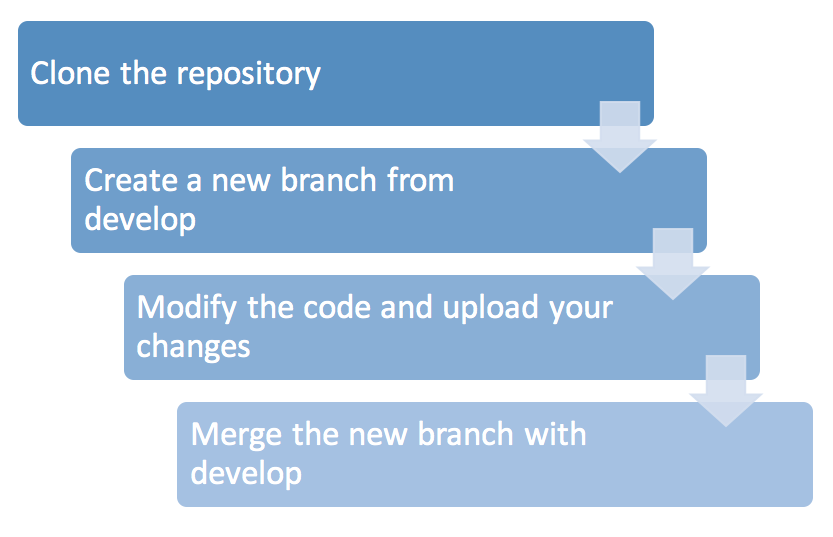
\includegraphics[width=12cm]{img/scheme_contributing.png}
	\caption{Scheme for contributing to AMIDST toolbox.}
	\label{fig:scheme_contributing}	
\end{figure}


\noindent Now we will explain each of these steps and the involved
commands.\newline 



\subsection{Clone the repository}\label{clone-the-repository}

First, you can download the source code from github using the following
command:

\begin{verbatim}
$ git clone https://github.com/amidst/toolbox.git      
\end{verbatim}

\noindent Once the download has finished, enter into the downloaded
folder:\newline

\begin{verbatim}
$ cd toolbox     
\end{verbatim}



\subsection{Create a new branch from develop }\label{create-a-new-branch-from-develop}

All the new development will be done in the branch develop. \textbf{Do not
modify the master branch} because it should always contain the source of
the very last release. Thus we change into the develop branch with the
following command:

\begin{verbatim}
$ git checkout develop    
\end{verbatim}

\noindent The terminal replies with the following output:

\begin{verbatim}
Checking out files: 100% (469/469), done.
Branch develop set up to track remote branch develop from origin.
Switched to a new branch 'develop'
\end{verbatim}

To avoid overlapping, we advise you to perform all your developments or
changes in a new branch created from develop. The name of this new
branch will be newfeature and it can be created with the following
command

\begin{verbatim}
$ git branch newfeature  
\end{verbatim}

\noindent We move into the recently created branch:\newline 

\begin{verbatim}
$ git checkout newfeature  
\end{verbatim}

\begin{verbatim}
Switched to branch 'newfeature'
\end{verbatim}



At any moment, we can verify which is the current branch with the
command show below. Make sure that your current branch is always the one you have created.

\begin{verbatim}
$ git branch
\end{verbatim}



\noindent Previous command shows a list with all the local branches, being the current
branch the one with the symbol *, for example:


\begin{verbatim}
develop
master
* newfeature
\end{verbatim}

\noindent The new branch is not yet a remote branch. For uploading it to the
server, we will use the following command:

\begin{verbatim}
$ git push --set-upstream origin newfeature
\end{verbatim}



\begin{verbatim}
Total 0 (delta 0), reused 0 (delta 0)
To https://github.com/amidst/toolbox.git
* [new branch]      newfeature -> newfeature
Branch newfeature set up to track remote branch newfeature from origin.
\end{verbatim}


\subsection{Modify the code and upload your changes }\label{modify-the-code-and-upload-your-changes}

As an example, we will simply create a new text file and upload it to
the server. For creating such file run:

\begin{verbatim}
$ echo "file to be deleted" > newfile.txt
\end{verbatim}


\noindent Now, we have to set the new file as a tracked file, for that
purpose:\newline 

\begin{verbatim}
$ git add newfile.txt 
\end{verbatim}


\noindent Which generates the output shown below indicating which of the tracked
files contain changes to be committed\newline

\begin{verbatim}
$ git status
\end{verbatim}


\noindent that generates the following output:

\begin{verbatim}
On branch newfeature
Your branch is up-to-date with 'origin/newfeature'.
Changes to be committed:
(use "git reset HEAD <file>..." to unstage)

new file:   newfile.txt

Untracked files:
(use "git add <file>..." to include in what will be committed)

...
\end{verbatim}


\noindent Now we will do a commit including the message ``added newfile.txt'' with
the following command:\\

\begin{verbatim}
$ git commit -m "added newfile.txt"
\end{verbatim}


\begin{verbatim}
[newfeature f256d1e] added newfile.txt
1 file changed, 1 insertion(+)
create mode 100644 newfile.txt
\end{verbatim}


\noindent Finally, we have upload all the changes to the server:\\

\begin{verbatim}
$ git push
\end{verbatim}



\subsection{Merge the new branch with develop }\label{merge-the-new-branch-with-develop}

Until now, the changes done are only present in the branch newfeature.
However, we should integrate these changes with the develop branch.
Thus, we first change to the branch develop:\\

\begin{verbatim}
$ git checkout develop
\end{verbatim}


\noindent Now, we will merge both branches:\\

\begin{verbatim}
$ git merge newfeature
\end{verbatim}


\noindent If there is not conflicts, an output similar to the following one will
be generated:\\

\begin{verbatim}
Updating 20ff914..f256d1e
Fast-forward
newfile.txt | 1 +
1 file changed, 1 insertion(+)
create mode 100644 newfile.txt
\end{verbatim}

\noindent Finally, we will upload the result of merging both branches to the
server:\\
\begin{verbatim}
$ git push
\end{verbatim}



\noindent Now, if we go to the AMIDST github website
(\url{https://github.com/amidst/toolbox}), we can verify that the branch
develop contains the changes in the code:


\begin{figure}[h!]
	\centering
	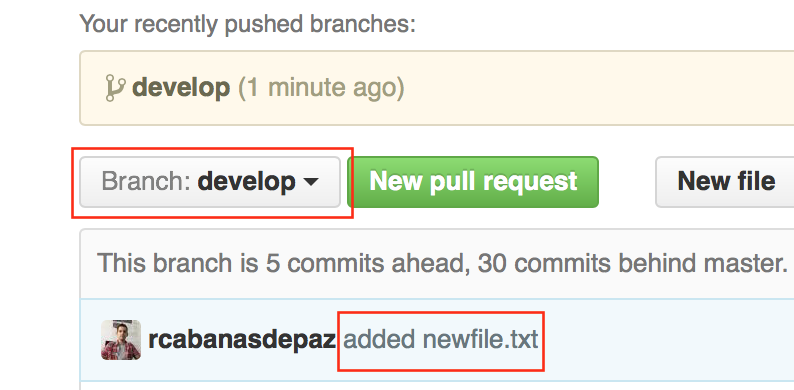
\includegraphics[width=10cm]{img/merge_result.png}
	\caption{View of the result of the contribution in the github website.}
	\label{fig:merge_result}	
\end{figure}

\end{document}